Three classifiers, including CNN, SVM, and \textit{k}NN were modeled in this work. All the three classifiers were modeled to classify the samples for different classification outputs. This section details how the classifiers were built and what hyper-parameters were used and optimized.
\subsection{Convolutional neural network}
Deep learning has been applied to many research areas and has achieved quite remarkable results. CNNs are widely used in image recognition and classification due to their power of automatically learning hierarchical representations directly from the raw data input. In this research, each spectrogram can be considered as an image with one channel. So a CNN is suitable to be applied into human recognition and activity classification using the spectrograms.

CNNs are a variant of artificial neural networks because they present a hierarchical sequence of convolutional layers alternated by pooling layers before the fully-connected layer of a regular neural network. A convolutional layer allows the network to detect spatial patterns over different parts of the input, and a pooling layer to learn translational invariance of the input. A typical CNN is depicted in Fig. \ref{fig_cnn}, where the \textit{Input} represents the dataset the network takes in, the \textit{Convolution} and \textit{Subsampling} (pooling function) are the operations performed on the data, the \textit{Feature maps} are the intermediate set of outputs; and the \textit{Output} is the final set of outputs. The unique architectural configuration of a CNN is defined by its \textit{hyperparameters}, whose values are set before the network is trained. An instance of a convolutional network is defined by its parameters whose values are learned during the network training \cite{bergado2018recurrent}.
\begin{figure}[!t]
\centering
%\captionsetup{justification=centering}
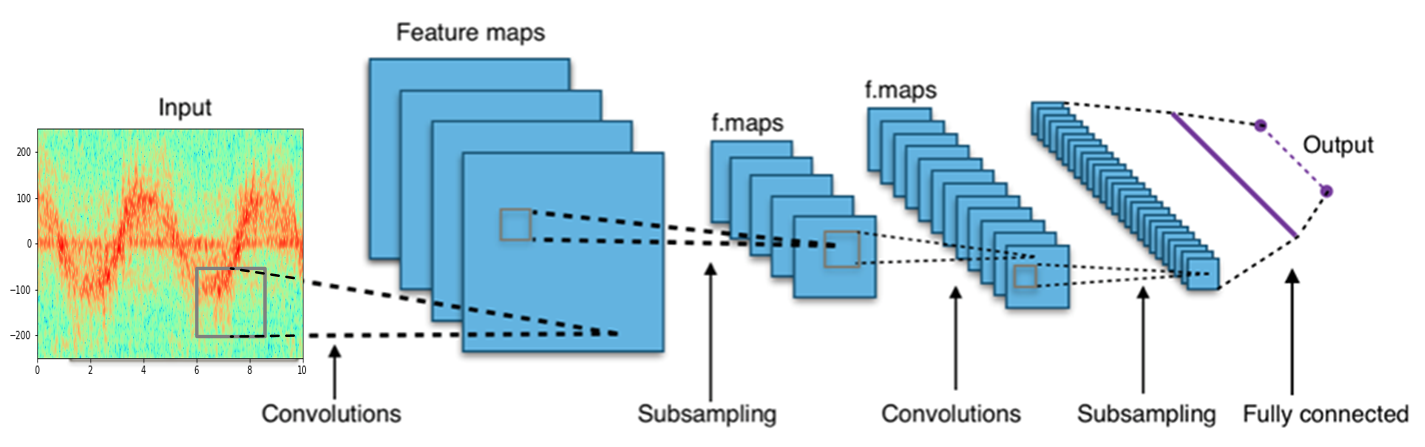
\includegraphics[width=3.6in]{cnn}
\caption{The structure of a CNN}
\label{fig_cnn}
\end{figure}

The next subsections describe details of the input, operations, and the output of a CNN making reference how it is applied to micro-Doppler signatures. We also detail how training and regularization are performed. Finally, we describe our proposed CNN architecture, called RadarNet, to perform the classification of the micro-Doppler signatures.
\subsubsection{Input}
The input in a CNN can be a full image or a set of it \cite{bergado2018recurrent}. An image is defined by its size, which is the height (number of rows) and width (number of columns) of its array of pixels and the number of channels ($C$) that are the different colors of the pixels (red, green and blue). Assuming $N$ is the number of images processed in parallel by the network and the image size as $H\times W$, a CNN input could be defined as an array $N\times H\times W\times C$. As described in section IV, a sequence of 2500 signal samples of one radar is transformed into a frequency spectrogram with the size of $2048 \times 304 \times 1$ (2048 is the height, 304 is the width, 1 is the depth), therefore the frequency spectrogram can be taken as an image with one channel.

\subsubsection{Operations}
A \textit{convolutional layer} is the main fundamental layer of a CNN. Each convolutional layer performs an aggregational operation aimed to learn the feature representation of the input (in our case spectrograms) and reduce the number of learnable parameters; it operates on the input/feature maps by applying a filter (e.g. kernel function) over the input. A convolution applies a linear operation on the input/feature maps using a set of filters $F$. The filter size is a matrix $G\times G$ of learnable parameters, on an input feature map $x$, it produces an output feature map $x^{'}$ as
\begin{equation}
\begin{split}
x^{'}=\sum_{i=1}^{k}\sum_{r=1}^{G}\sum_{c=1}^{G}x_{rc}\cdot F_{i}+b^{'}
\end{split}
\end{equation}
where $k$ is the number of filters $F$, $b^{'}$ is the bias parameter associated with the feature map $x^{'}$.

By convolving the input with the filter, a set of feature maps is produced. A convolutional layer is parameterized by a \textit{depth}, a \textit{kernel field size}, a \textit{stride}, and a \textit{zero-padding}. The depth determines the channel size of the output (i.e. the desired number of feature maps). The kernel field size, i.e. the filter size, covers a small region of pixels of the input image at each convolution step (see the red square in Fig. \ref{fig_convol}). Each element in a feature map is generated by the filter convolving with the covered region of the input (e.g. the generated elements in the yellow feature map in Fig. \ref{fig_convol}). The stride determines the number of pixels by the filter which is moved during each filtering step over the image. As can be seen in Fig. \ref{fig_convol} by the red and purple squares (representing the filter) over the Input image. The zero-padding is used to pad the input with zeros on its border, as seen in Fig. \ref{fig_convol}. The zero-padding is useful to determine a desired output size of the feature map. For example, given an input image of height and width  $H\times W$, a kernel field size of $G\times G$, a stride $S$, and an amount of zero padding $P$, the spatial size ($H{'}\times W{'}$) of the feature map generated can be computed as  \cite{bergado2018recurrent}: 
\begin{equation}
\begin{split}
H{'}=(H-G+2P)/S+1,\\
W{'}=(W-G+2P)/S+1
\end{split}
\end{equation}


Fig. \ref{fig_convol} provides a numerical example of the convolution process: assuming an image with the size of $4\times 4$ pixels that is zero-padded with value $1$, then convolutionalized by a kernel of $3\times 3$ with a stride of $2$, a resulting feature map of $2\times 2$ neurons is produced.  
\begin{figure}[!t]
\centering
%\captionsetup{justification=centering}
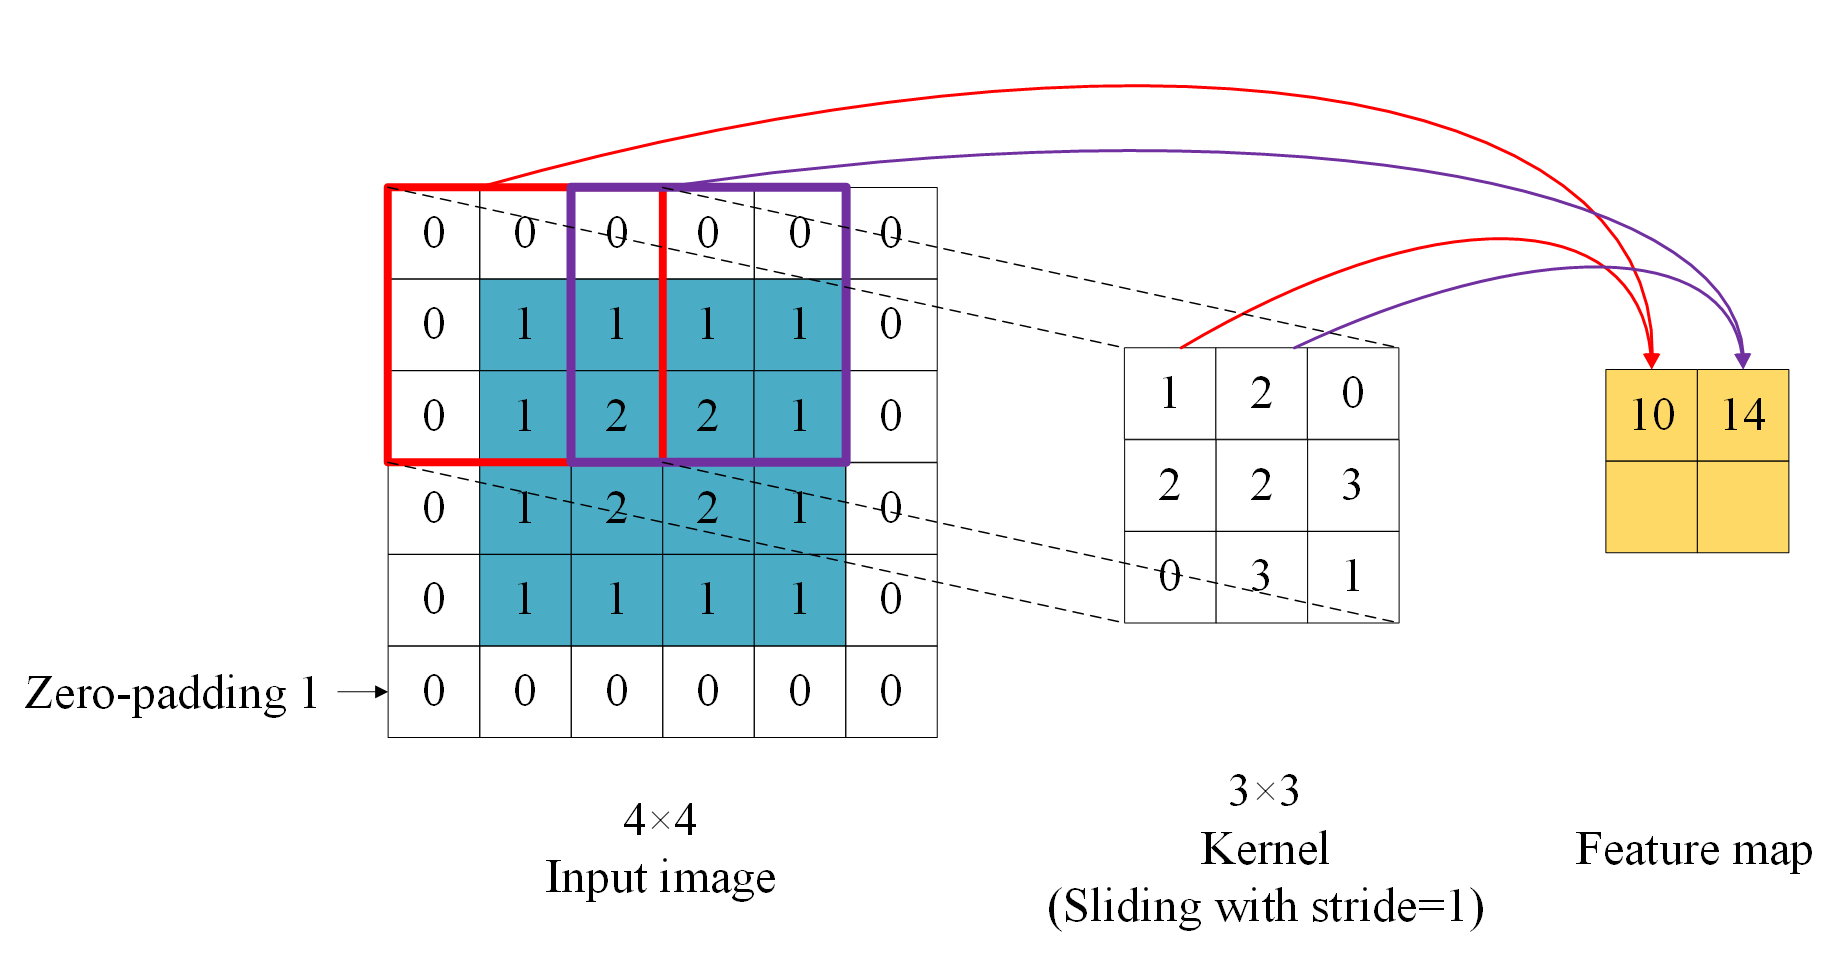
\includegraphics[width=3.6in]{convolution}
\caption{Convolution process}
\label{fig_convol}
\end{figure}

The \textit{pooling layer} is a form of non-linear down-sampling. It is designed to reduce the spatial size (dimensionality) of the input, in order to reduce the number of parameters (e.g. neurons and their connectivity) in the CNN. It aggregates the values of a local region of the input (window), commonly by applying an average or a maximum function.  Max pooling is the most common function to implement pooling by using the maximum function. It partitions the input image into a set of non-overlapping windows (e.g. the red bordered square in Fig. \ref{fig_pool}). For each such window, it takes the maximum neuron value of that window and places it as an output neuron (as shown in Fig. \ref{fig_pool}, where the resulting maximum value is 8 of the bordered red square). It is common to periodically insert a pooling layer between successive convolutional layers in a CNN architecture.  A complete Max-pooling operation is shown in Fig. \ref{fig_pool} for an input matrix of $4\times 4$ that is reduced to a $2\times 2$ matrix size, by using a $2\times 2$ sliding window and taking the maximum value of each window.
\begin{figure}[!t]
\centering
%\captionsetup{justification=centering}
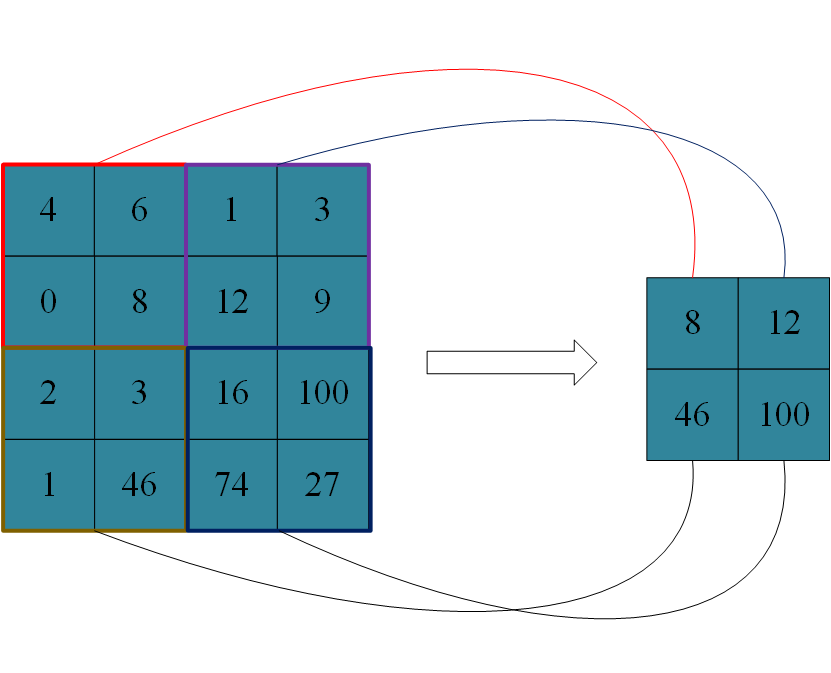
\includegraphics[width=2.6in]{pooling}
\caption{Max-pooling operation}
\label{fig_pool}
\end{figure}

\textit{Fully connected layers} can be seen as regular neural network layers. All neurons in the previous layer are transformed into a one-dimensional vector in a fully connected layer. Fully connected layers are added after all convolutional layers and pooling layers.

An \textit{activation layer} is not a typical layer in CNNs, but it is a nonlinearity operation commonly used in neural networks. It increases the nonlinear properties of CNNs. As the result of a series of linear operations (like convolutions) can be a single-linear operation, an elementwise nonlinear function can be applied between convolutions in order to introduce nonlinearity \cite{bergado2018recurrent}. This makes CNNs capable to learn more complex mappings of input to output. The activation function used in our work is the ReLU (Rectified Linear Units) \cite{nair2010rectified}, which is formulated as:
\begin{equation}
f(x)=Max(0,x),
\end{equation}
Other functions are also used to increase nonlinearity, such as
\begin{equation}
\begin{split}
\text{sigmoid}: f(z)=1/(1+\exp(-z) ),\\
\text{tanh}: f(z)=\tanh(z)=\frac{e^z-e^{(-z)}}{e^z+e^{(-z)}}
\end{split}
\end{equation}

ReLU is often preferred over other functions because it trains the neural network several times faster without a significant penalty to the generalization accuracy.
\subsubsection{Output}
The Feature maps are intermediary outputs of a CNN layer and at the same time input to the next layer. In CNNs, the final outputs comprise of final score maps, which represent the probabilities of each input element belonging to a label. The calculated accuracy is in relation to the final score maps and the reference labels.
\subsubsection{The Network Training Process}
The model is trained to minimize an objective function in terms of the parameters of the network. For a given classification, let $C$ be the number of labeled classes, the following cross-entropy loss function \cite{de2005tutorial} is often used:
\begin{equation}
E_y (y^{'} )=-\sum_{i=1}^{N}y_i\cdot log(y_i^{'})
\end{equation}
where $E$ is the loss function evaluated over $N$ samples, $y_i$ is the original label of the $i_{th}$ sample and $y_i^{'}$ is the class score maps of a sample $i$ calculated using a \textit{softmax} activation function \cite{dunne1997pairing}:
\begin{equation}
y_j=exp(x_j)/(\sum_{c=1}^{C}exp(x_c))
\end{equation}
where $y$ is the softmax score and $x$ is the output layer containing unnormalized class scores.

In order to minimize the objective function, a backpropagation with gradient descent is normally applied. Computing the gradient yields to:
\begin{equation}
\partial E/\partial y_i =-y_i^{'}/y_i 
\end{equation}
\begin{equation}
\begin{split}
\partial y_i/\partial x_k&=\left\{\begin{matrix}
\frac{e^{x_i}}{\sum_{c=1}^{C}e^{x_c}}-(\frac{e^{x_i}}{\sum_{c=1}^{C}e^{x_c}})^2 & i=k\\ 
-(\frac{e^{x_i}e^{x_k}}{\sum_{c=1}^{C}e^{x_c}})^2
& i\neq k
\end{matrix}\right. \\
&=\left\{\begin{matrix}
y_i(1-y_i)) &i=k \\ 
 -y_iy_k& i\neq k
\end{matrix}\right.
\end{split}
\end{equation}
\begin{equation}
\begin{split}
\partial E/\partial x_i&=\sum_{k=1}^{C}(\partial E/\partial y_k)(\partial y_k/\partial x_i) \\&=
\frac{\partial E}{\partial y_i} \frac{\partial y_i}{\partial x_i}-\sum_{k\neq 1}^{C}\frac{\partial E}{\partial y_k}\frac{\partial y_k}{\partial x_i}\\&=-y_i^{'}(1-y_i)+\sum_{k\neq 1}y_k^{'}y_i\\&=-y_i^{'}+y_i\sum_{k\neq 1}y_k^{'}\\&=y_i-t_i
\end{split}
\end{equation}

Then the partial derivative of the loss function with respect to convolutional kernels $w_{ji}$ connecting input unit $i$ to the hidden units in the top layer, indexed by $j$, has a gradient of
\begin{equation}
\partial E/\partial w_{ij}=\sum_{i=1}^{C}(\partial E/\partial x_i)(\partial x_i/\partial w_{ij})=(y_i-t_i)h_i
\end{equation}
For units $j$ in the hidden layer, we have
\begin{equation}
\begin{split}
\partial E/\partial x_{j}&=\sum_{i}(\partial E/\partial x_i)(\partial x_i/\partial h_j)(\partial h_j/\partial x_j)\\ &=\sum_{i=1}^{C}(y_i-t_i)(h_i(1-h_i))
\end{split}
\end{equation}

The iterative training rule for updating the network parameters $w_{ji}$ and hidden units $j$ through the gradient descent strategy is as follows:
\begin{equation}
\begin{matrix}
w_{ij}\leftarrow w_{ij}-\alpha \cdot (\partial E/\partial w_{ij})\\ 
x_j\leftarrow x_j-\alpha \cdot (\partial E/\partial x_{j})
\end{matrix}
\end{equation}
where $\alpha$ is the learning rate for the whole network, it is a hyperparameter that is required to be initialized before the training.

\subsubsection{Regularization of CNNs}
Regularization are techniques used to address the problem of overfitting in statistical models. Overfitting occurs in deep learning when a CNN model classifies with high accuracy during training but presents poor classification accuracy in unseen test data. Overfitting is normally due to the rare dependencies in the training data that may not occur in the overall population.  The most common regularization methods are: \textit{data augmentation, early stopping, dropout and weight decay}. \textit{Data augmentation} increases the number of training samples by introducing distortions in the original samples by permuting samples or applying translational transformations. The amount of distortion should still ensure the labelling of each new training sample is still valid, this allows a model to become more invariant to small changes in input and hence allow for better generalization of the CNN. \textit{Early stopping} is to stop the training process by monitoring the loss on the validation set in order to prevent the overfitting resulted by over-training. When the validation loss increases for a specified number of iterations, the training is stopped. \textit{Dropout} \cite{srivastava2014dropout} is a regularization method commonly used in neural networks. The term ``dropout`` refers to dropping out a part of the units in a neural network. By avoiding training all nodes on all training data, dropout decreases overfitting in neural networks. \textit{Weight decay} adds a penalty term by multiplying each weight in the gradient descent at each epoch with a factor $\lambda 
,(0<\lambda 
<1)$, in order to penalize large weights. With weight decay term, the $w_{ij}$ in 
\begin{equation}
w_{ij}\leftarrow w_{ij}-\alpha \cdot (\partial E/\partial w_{ij})-\alpha \cdot \lambda  w_{ij}
\end{equation}

\subsubsection{RadarNet – Our Proposed CNN}
Our radar system consists of two BumbleBee radars. Both of them detect the target at the same time. In order to fuse the signals from the radars, the spectrograms generated from them are firstly downsampled into the size of $50\times 50\times 1$, then overlapped together. The downsampling is achieved by resizing the spectrograms using bilinear interpolation algorithm. It is beneficial to accelerate the training phrase by reducing the number of parameters since the size of $2048\times 304\times 1$ is too large. The resulting overlapped spectrograms can be considered as images with two channels. As shown as Fig. \ref{fig_cnn_}, the overlapped spectrogram with the shape of $50\times 50\times 2$ is input into a CNN model, which is named `RadarNet`. RadarNet contains three convolutional layers (C1, C2, and C3), two Max Pooling layers (M1, M2) and two fully connected layers. All three convolutional layers use $3\times 3$ kernels to do the convolutionalization. The C1 layer contains $16$ feature maps, and the size of each feature map is $48\times 48\times 1$. A $2\times 2$ filter is used to perform the \textit{Max Pooling} on C1, and generate the M1 layer. The C2 layer contains $32$ feature maps, and the size of each feature map is $22\times 22\times 1$. The resulting M2 layer by Max-Pool the C2 layer has the size of $11\times 11\times 1$. The C3 layer contains 48 feature maps, each feature map is a $9\times 9\times 1$ matrix. The F1 layer contains 356 hidden units, and the F2 contains 160 hidden units.

In RadarNet, Dropout has been used to control overfitting with an initial dropout rate of 0.4. Batch normalization \cite{ioffe2015batch} has been applied on $M1$, $M2$, $F1$, and $F2$ as a regularizer to accelerate convergence. Batch normalization normalizes the output of a previous activation layer by subtracting the batch mean and dividing by the batch standard deviation. The Batch normalization is presented in Algorithm 1. In the algorithm, $\epsilon$ is a constant added to the mini-batch variance for numerical stability \cite{ioffe2015batch}.
\begin{algorithm}
 \caption{ Batch Normalization\cite{ioffe2015batch}.}  
  \label{alg:bn}  
\begin{algorithmic}[1]  
    \Require  
      Values of x over a mini-batch: $B={x_1…,x_m}$;
            Parameters to be learned: $\gamma$ , $\beta$  
    \Ensure   ${y_i=BN_{(\gamma,\beta)} (x_i)}$  
    \newline
    \\$\mu _B\leftarrow (1/m)\sum_{i=1}^{m}x_i$ \qquad $//$ min-batch mean 
 \newline
    \\$\sigma ^2 _B\leftarrow (1/m)\sum_{i=1}^{m}(x_i-\mu _B)^2$ \qquad $//$ min-batch variance
    \newline
    \\$\hat{x}_i\leftarrow (x_i-\mu _B)/\sqrt{\sigma ^2 _B+\epsilon }$ \qquad  $//$ normalize
    \newline
    \\$y_i\leftarrow \gamma \hat{x}_i+\beta \equiv BN_{(\gamma,\beta)} (x_i)$ \qquad $//$scale and shift

  \end{algorithmic}  
\end{algorithm}


The use of dropout and batch normalization reduces overfitting and accelerates the training. The optimization function applied is \textit{Adadelta}, whose initial learning rate is 0.1. Adadelta is an optimization function that can dynamically adapt over time using only first order information and it has minimal computational overhead beyond standard stochastic gradient descent, which is one of the most popular methods used to perform optimization. Adadelta requires no manual tuning of a learning rate and appears robust to noisy gradient information, different model architecture choices, various data modalities, and selection of hyperparameters \cite{zeiler2012adadelta}. 

RadarNet is used to perform human detection, activity classification, range estimation, and people counting. 
\begin{figure}[!t]
\centering
%\captionsetup{justification=centering}
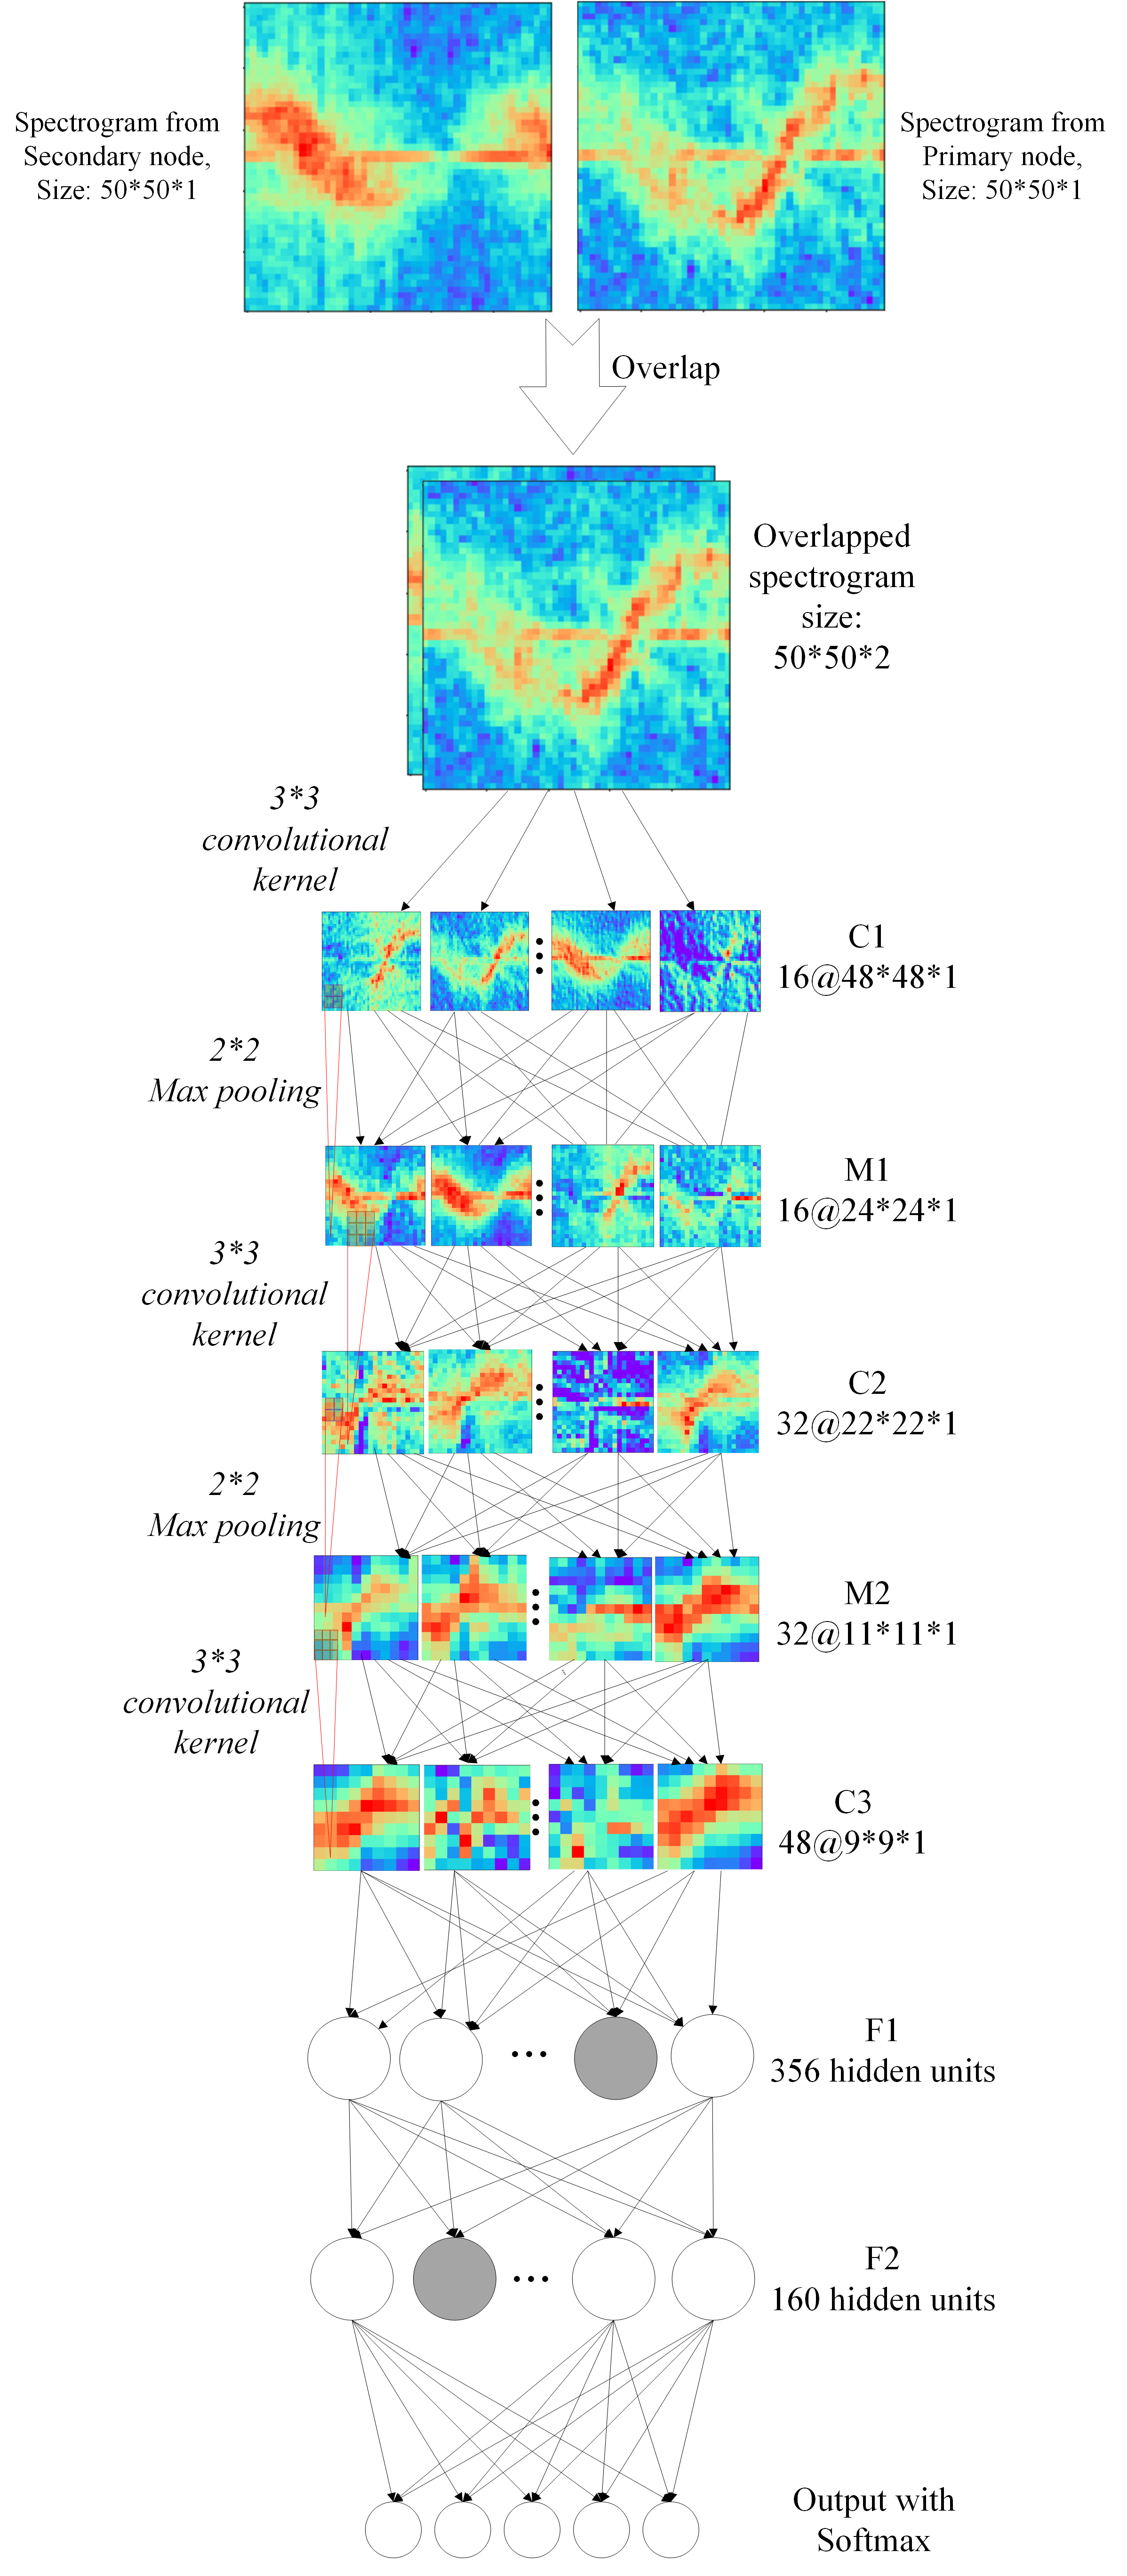
\includegraphics[width=3.6in]{cnn_}
\caption{Structure of the CNN in human behaviour detection}
\label{fig_cnn_}
\end{figure}

\subsection{Support vector machine}
As mentioned in Section I, SVM is one of the most used classifiers in micro-Doppler based human activity detection. SVMs are discrete algorithms that can be used to find the optimal separating hyperplane that maximizes the margin of the training data. A hyperplane is a decision boundary to separate data of different classes. As a dataset is usually non-linear separable in practice, the SVM algorithm is implemented using a kernel, which is a way of transforming the input data into a high-dimensional space. In the transformed feature space, it is possible to separate the data with a linear hyperplane.  An SVM with RBF (Radial basis function) kernel has been applied because a Linear SVM cannot separate the micro-Doppler data successfully.   

Differently from the works in \cite{narayanan2015radar,ccaugliyan2015micro,kim2009human,zenaldin2016radar} where the features fed into SVMs were handcrafted, the input features used in our work were extracted automatically in two ways. One way was to calculate the mean value of each column in each spectrogram and define it as a feature. Another way was applying 2D2PCA on the samples to extract the features. The results of these two feature extraction methods are compared.

Two hyperparameters $(C, gamma)$ in RBF SVM were specified manually. Cross-validation was used to tune the hyperparameters. Given a hyperparameter space  $C: [1,30],gamma:[0.1,1.0E-5]$, a different pair of parameters was selected from the hyperparameter space by the cross-validation in each training and validation iteration, in order to build a SVM classifier. The parameters that made the SVM to perform the best were considered as the optimal parameters. Table \ref{tb-svmhp} presents the optimal parameters for different classification tasks.
\begin{table}[]
\centering
\caption{Optimal hyperparameters for different classification tasks}
\label{tb-svmhp}
\begin{tabular}{|c|c|c|c|}
\hline
\textbf{Task}                                  & \textbf{Model} & \textbf{Gamma} & \textbf{C} \\ \hline
\multirow{2}{*}{Human recognition}             & SVM            & 1.0E -3.57     & 7          \\ \cline{2-4} 
                                               & SVM+2D2PCA     & 1.0E -5.84     & 3.1        \\ \hline
\multirow{2}{*}{Human activity classification} & SVM            & 1.0E -3.35     & 7.34       \\ \cline{2-4} 
                                               & SVM+2D2PCA     & 1.0E -5.67     & 5.37       \\ \hline
\multirow{2}{*}{People counting}               & SVM            & 1.0E -3.26     & 6          \\ \cline{2-4} 
                                               & SVM+2D2PCA     & 1.0E -6        & 6.5        \\ \hline
\multirow{2}{*}{Coarse-grained localization}   & SVM            & 1.0E -3.57     & 7.9        \\ \cline{2-4} 
                                               & SVM+2D2PCA     & 1.0E -6.07     & 2.9        \\ \hline
\end{tabular}
\end{table}

\subsection{\textit{k}--Nearest--Neighbor}
The \textit{k-Nearest-Neighbor} (\textit{k}NN) classification is one of the most fundamental and simple classification methods and should be one of the first choices for a classification study when there is little or no prior knowledge about the distribution of the data \cite{peterson2009k}. It also has been widely used in micro-Doppler based human activity detection\cite{ccaugliyan2015micro,erol2015kinect,gurbuz2015operational}. The \textit{k}NN classification algorithm itself is fairly straightforward and it can be summarized by the following steps: 
\begin{enumerate}
\item Choose the number for \textit{k} and a distance metric, which is commonly based on the Euclidean distance.
\item Find the \textit{k} nearest neighbors of the sample that needs to be classified
\item Assign a class label by majority vote.
\end{enumerate}

In human activity classification,  a set of features extracted from frequency spectrograms of a micro-Doppler radar can be represented by $\{f_j\}_M^N, (1 \leq j\leq M)$. Where $N$ is the number of labelled samples (frequency spectrograms),  $M$ is the number of features in each sample,  $f_j$ is the $j_{th}$ feature, and an un-labelled sample can be represented $S_i=〖\{f_j^i\} 〗_M, (1\leq j\leq M)$. In order to find $k$ closest samples to $S_i$, it is necessary to calculate the distance between each lablled sample $S_c, (1 \leq c\leq N)$ and $S_i$. A possible way to calculate this distance is using the Euclidean distance as follows:
\begin{equation}
\begin{split}
Dist(S_c,S_i)&=Dist((f_1^c,…,f_M^c ),(f_1^i,\ldots,f_M^i ))\\&=\sqrt{\sum_{p=1}^{M} (f_p^c-f_p^i)^2}
\end{split}
\end{equation}

Cross-validation is used to select a value of  \textit{k} that minimizes the overall distance between the  \textit{k} nearest labelled samples and the un-labelled sample. Finally, the unlabeled sample will be classified to the class label with a majority vote from the  \textit{k} nearest labelled samples. For each classification task, the chosen value of  \textit{k} is presented in Table \ref{tb-knn}.
% Please add the following required packages to your document preamble:
% \usepackage{multirow}
\begin{table}[]
\centering
\caption{The value \textit{k} of \textit{k}NN in different Task}
\label{tb-knn}
\begin{tabular}{|c|c|c|}
\hline
\textbf{TASK}                                  & \textbf{MODEL} & \textbf{K} \\ \hline
\multirow{2}{*}{Human recognition}             & kNN            & 1          \\ \cline{2-3} 
                                               & kNN+2D2PCA     & 1          \\ \hline
\multirow{2}{*}{Human activity classification} & KNN            & 9          \\ \cline{2-3} 
                                               & kNN+2D2PCA     & 5          \\ \hline
\multirow{2}{*}{People counting}               & KNN            & 4          \\ \cline{2-3} 
                                               & kNN+2D2PCA     & 1          \\ \hline
\multirow{2}{*}{Coarse-grained localisation}   & KNN            & 7          \\ \cline{2-3} 
                                               & kNN+2D2PCA     & 1          \\ \hline
\end{tabular}
\end{table}